\section{Overall Description}

\subsection{User needs}

\begin{content}
ECAP5 is the primary user for ECAP5-DPROC. ECAP5-DPROC could however be used as a standalone RISC-V processor. The following requirements define the user needs. 
\end{content}

\ureq{U\_INSTRUCTION\_SET\_01}{
  ECAP5-DPROC shall implement the RV32I instruction set.
}

\begin{content}
  In order to improve the usability of ECAP5-DPROC, it shall have a \textit{von Neumann} architecture as it only requires one memory interface.
\end{content}

\ureq{U\_MEMORY\_INTERFACE\_01}{
  ECAP5-DPROC shall access both instructions and data through a unique memory interface.
}

\ureq{U\_MEMORY\_INTERFACE\_02}{
  ECAP5-DPROC's unique memory interface shall be compliant with the AXI-Lite specification.
}

\ureq{U\_MEMORY\_INTERFACE\_03}{
  ECAP5-DPROC's unique memory interface shall be designed such that memory protocols can be interchanged at compile time.
}

\ureq{U\_RESET\_01}{
  ECAP5-DPROC shall provide a signal which shall hold ECAP5-DPROC in a reset state while asserted.
}

\begin{content}
The polarity of the reset signal mentionned in \texttt{U\_RESET\_01} is not specified by the user.
\end{content}

\ureq{U\_BOOT\_ADDRESS\_01}{
  The address at which ECAP5-DPROC jumps after the reset signal is deasserted shall be hardware-configurable.
}

\begin{content}
The address mentionned in \texttt{U\_BOOT\_ADDRESS\_01} can be either configured through hardware signals or can be selected at compile time.
\end{content}

\ureq{U\_HARDWARE\_INTERRUPT\_01}{
  ECAP5-DPROC shall provide an signal which shall interrupt ECAP5-DPROC's execution flow while asserted.
}

\ureq{U\_HARDWARE\_INTERRUPT\_02}{
  ECAP5-DPROC shall jump to a software-configurable address when it is interrupted.
}

\begin{content}
The memory address at which ECAP5-DPROC shall jump to when interrupted is not specified by the user.
\end{content}

\ureq{U\_DEBUG\_01}{
  ECAP5-DPROC shall be compliant with the RISC-V External Debug Support specification.
}

\begin{content}
There is no performance goal required by ECAP5 for ECAP5-DPROC as ECAP5 is an educational platform.
\end{content}

\subsection{Assumptions and Dependencies}

\begin{content}
Describe what the assumptions for the product are : Targeting the ecp5 family, based around opensource toolchains.
\end{content}

\section{Requirements}

\subsection{External Interface Requirements}

\begin{figure}[h!]
    \centering
    \scalebox{0.85}{
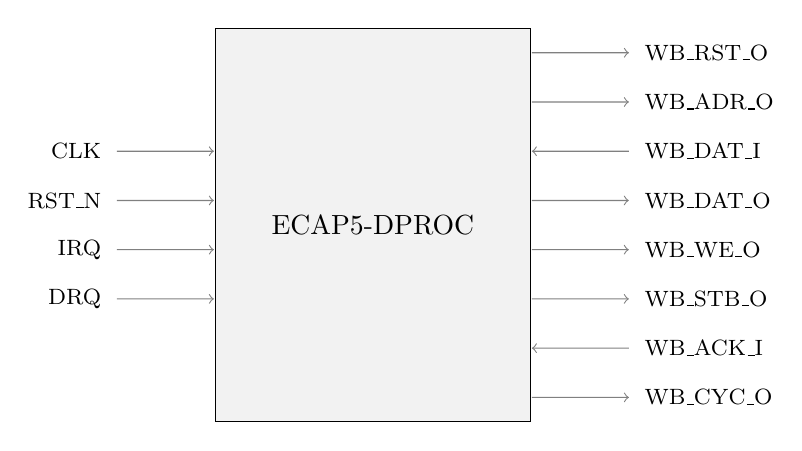
\begin{tikzpicture}[scale=1.25, draw=gray, inner sep=0, outer sep=0]
  \node[rectangle, draw=black,
    minimum height = 5cm,
    minimum width = 4cm,
    fill = gray!10] (box) at (0, 0) {ECAP5-DPROC};

  % left
  \node (lport1) at ([yshift=0.75cm]box.west) {};
  \node (lport2) at ([yshift=0.25cm]box.west) {};
  \node (lport3) at ([yshift=-0.25cm]box.west) {};
  \node (lport4) at ([yshift=-0.75cm]box.west) {};

  \draw[->] ([xshift=-1cm]lport1.center) node[left=0.2cm, anchor=east]{\footnotesize CLK} -- (lport1);
  \draw[->] ([xshift=-1cm]lport2.center) node[left=0.2cm, anchor=east]{\footnotesize RST\_N} -- (lport2);
  \draw[->] ([xshift=-1cm]lport3.center) node[left=0.2cm, anchor=east]{\footnotesize IRQ} -- (lport3);
  \draw[->] ([xshift=-1cm]lport4.center) node[left=0.2cm, anchor=east]{\footnotesize DRQ} -- (lport4);

  % right
  \node (rport4) at ([yshift=0.25cm]box.east) {};
  \node (rport3) at ([yshift=0.5cm]rport4.center) {};
  \node (rport2) at ([yshift=0.5cm]rport3.center) {};
  \node (rport1) at ([yshift=0.5cm]rport2.center) {};

  \node (rport5) at ([yshift=-0.25cm]box.east) {};
  \node (rport6) at ([yshift=-0.5cm]rport5.center) {};
  \node (rport7) at ([yshift=-0.5cm]rport6.center) {};
  \node (rport8) at ([yshift=-0.5cm]rport7.center) {};

  \draw[<-] ([xshift=1cm]rport1.center) node[right=0.2cm, anchor=west]{\footnotesize WB\_RST\_O} -- (rport1);
  \draw[<-] ([xshift=1cm]rport2.center) node[right=0.2cm, anchor=west]{\footnotesize WB\_ADR\_O} -- (rport2);
  \draw[->] ([xshift=1cm]rport3.center) node[right=0.2cm, anchor=west]{\footnotesize WB\_DAT\_I} -- (rport3);
  \draw[<-] ([xshift=1cm]rport4.center) node[right=0.2cm, anchor=west]{\footnotesize WB\_DAT\_O} -- (rport4);
  \draw[<-] ([xshift=1cm]rport5.center) node[right=0.2cm, anchor=west]{\footnotesize WB\_WE\_O} -- (rport5);
  \draw[<-] ([xshift=1cm]rport6.center) node[right=0.2cm, anchor=west]{\footnotesize WB\_STB\_O} -- (rport6);
  \draw[->] ([xshift=1cm]rport7.center) node[right=0.2cm, anchor=west]{\footnotesize WB\_ACK\_I} -- (rport7);
  \draw[<-] ([xshift=1cm]rport8.center) node[right=0.2cm, anchor=west]{\footnotesize WB\_CYC\_O} -- (rport8);
\end{tikzpicture}
}

    \caption{Schematic view of the external interface of ECAP5-DPROC}
    \label{fig:externalinterface}
\end{figure}

\begin{table}[H]
  \centering
  {
\footnotesize
\begin{tabularx}{0.9\textwidth}{|l|c|c|X|}
  \hline
  \cellcolor{gray!20}\textbf{NAME} & \cellcolor{gray!20}\textbf{TYPE} & \cellcolor{gray!20}\textbf{WIDTH} & \cellcolor{gray!20}\textbf{DESCRIPTION} \\
  \hline
  CLK & I & 1 & Clock input. \\
  \hline
  RST\_N & I & 1 & Hardware reset. Active low. \\
  \hline
  IRQ & I & 1 & External interrupt request. \\
  \hline
  DRQ & I & 1 & Debug request. \\
  \hline
\end{tabularx}
}

  \caption{ECAP5-DPROC control signals}
  \label{tab:control-interface}
\end{table}

\begin{table}[H]
  \centering
  {
\footnotesize
\begin{tabularx}{0.9\textwidth}{|l|c|c|X|}
  \hline
  \cellcolor{gray!20}\textbf{NAME} & \cellcolor{gray!20}\textbf{TYPE} & \cellcolor{gray!20}\textbf{WIDTH} & \cellcolor{gray!20}\textbf{DESCRIPTION} \\
  \hline
  \multicolumn{4}{|l|}{\textbf{READ ADDRESS BUS}} \\
  \hline
  ARADDR & O & 32 & Read address. \\
  \hline
  ARVALID & O & 1 & Read address valid. \\
  \hline
  ARREADY & I & 1 & Read address ready. \\ 
  \hline
  \multicolumn{4}{|l|}{\textbf{READ DATA BUS}} \\
  \hline
  RDATA & I & 32 & Read data. \\
  \hline
  RRESP & I & 2 & Read response. \\
  \hline
  RVALID & I & 1 & Read valid. \\
  \hline
  RREADY & O & 1 & Read ready. \\ 
  \hline
  \multicolumn{4}{|l|}{\textbf{WRITE ADDRESS BUS}} \\
  \hline
  AWADDR & O & 32 & Write address. \\
  \hline
  AWVALID & O & 1 & Write address valid. \\
  \hline
  AWREADY & I & 1 & Write address ready \\
  \hline
  \multicolumn{4}{|l|}{\textbf{WRITE DATA BUS}} \\
  \hline
  WDATA & O & 32 & Write data. \\
  \hline
  WSTRB & O & 4 & Write strobes. \\
  \hline
  \multicolumn{4}{|l|}{\textbf{WRITE RESPONSE BUS}} \\
  \hline
  BRESP & I & 2 & Write response. \\
  \hline
  BVALID & I & 1 & Write response valid. \\
  \hline
  BREADY & O & 1 & Response ready. \\
  \hline
\end{tabularx}
}

  \caption{ECAP5-DPROC memory interface signals}
  \label{tab:memory-interface}
\end{table}

\ireq{I\_CLK\_01}{
  All inputs and outputs of ECAP5-DPROC shall belong to CLK's clock domain.
}{}

\ireq{I\_RESET\_01}{
  The RST\_N signal shall hold ECAP5-DPROC in a reset state while asserted.
}{
  U\_RESET\_01
}

\ireq{I\_RESET\_02}{
  RST\_N polarity shall be active low.
}{}

\ireq{I\_IRQ\_01}{
  ECAP5-DPROC shall jump to a software-configurable address when input IRQ is asserted.
}{
  U\_HARDWARE\_INTERRUPT\_01, U\_HARDWARE\_INTERRUPT\_02
}

\ireq{I\_DIRQ\_01}{
  TBD
}{}

\ireq{I\_MEMORY\_INTERFACE\_01}{
  Signals from table \ref{tab:memory-interface} shall be compliant with the AXI-Lite specification.
}{
  U\_MEMORY\_INTERFACE\_02
}

\begin{content}
  Behavioral specification for symbols in table \ref{tab:memory-interface} is outlined in the functional requirements section, subsection \ref{spec-memory-interface}.
\end{content}

\subsection{Functional Requirements}

\subsubsection{Register file}

\req{F\_REGISTERS\_01}{
  ECAP5-DPROC shall implement 31 user-accessible general purpose registers ranging from \texttt{x0} to \texttt{x31}.
}{U\_INSTRUCTION\_SET\_01}

\req{F\_REGISTERS\_02}{
  Register \texttt{x0} shall be hardwired to the constant zero.
}{U\_INSTRUCTION\_SET\_01}

\req{F\_REGISTERS\_03}{
  ECAP5-DPROC shall implement a \texttt{pc} user-accessible register storing the address of the current instruction.
}{U\_INSTRUCTION\_SET\_01}

\subsubsection{Instruction decoding}

\begin{content}
  Figure \ref{fig:instructionencoding} outlines the different instruction encodings for the RV32I instruction set. The \texttt{opcode} parameter is a unique identifier for each instruction. The instruction encoding is infered from the opcode as there can only be one encoding per opcode.
\end{content}

\begin{figure}[h!]
    \centering
    \vspace{0.5em}

\hspace{2em}
\scalebox{0.9}{
\begin{bytefield}[
    bitwidth=1.1em, 
    endianness=big, 
    bitformatting={\scriptsize}, 
    boxformatting={\centering\footnotesize\ttfamily},
    rightcurly=., rightcurlyspace=5pt
]{32}
  \bitheader{0,6,7,8,11,12,14,15,19,20,24,25,31} \\
  \begin{rightwordgroup}{\footnotesize R-type}
    \bitbox{7}{funct7}
    \bitbox{5}{rs2}
    \bitbox{5}{rs1}
    \bitbox{3}{func3}
    \bitbox{5}{rd}
    \bitbox{7}{opcode}
  \end{rightwordgroup}
  \\[2ex]
  \begin{rightwordgroup}{\footnotesize I-type}
    \bitbox{12}{imm[11:0]}
    \bitbox{5}{rs1}
    \bitbox{3}{func3}
    \bitbox{5}{rd}
    \bitbox{7}{opcode}
  \end{rightwordgroup}
  \\[2ex]
  \begin{rightwordgroup}{\footnotesize S-type}
    \bitbox{7}{imm[11:5]}
    \bitbox{5}{rs2}
    \bitbox{5}{rs1}
    \bitbox{3}{func3}
    \bitbox{5}{imm[4:0]}
    \bitbox{7}{opcode}
  \end{rightwordgroup}
  \\[2ex]
  \begin{rightwordgroup}{\footnotesize B-type}
    \bitbox{1}{a}
    \bitbox{6}{imm[10:5]}
    \bitbox{5}{rs2}
    \bitbox{5}{rs1}
    \bitbox{3}{func3}
    \bitbox{4}{imm[4:1]}
    \bitbox{1}{b}
    \bitbox{7}{opcode}
  \end{rightwordgroup}
  \\[2ex]
  \begin{rightwordgroup}{\footnotesize U-type}
    \bitbox{20}{imm[31:12]}
    \bitbox{5}{rd}
    \bitbox{7}{opcode}
  \end{rightwordgroup}
  \\[2ex]
  \begin{rightwordgroup}{\footnotesize J-type}
    \bitbox{1}{c}
    \bitbox{10}{imm[10:1]}
    \bitbox{1}{b}
    \bitbox{8}{imm[31:12]}
    \bitbox{5}{rd}
    \bitbox{7}{opcode}
  \end{rightwordgroup}
\end{bytefield}
}

\vspace{0.25em}
\scalebox{0.7}{
\begin{tabularx}{0.8\textwidth}{Y Y Y}
a: \texttt{imm[12]} & b: \texttt{imm[11]} & c: \texttt{imm[20]}
\end{tabularx}
}

    \caption{Instruction encodings of the RV32I instruction set}
    \label{fig:instructionencoding}
\end{figure}

\paragraph{Immediate encoding}

\begin{content}
  Only one immediate value can be encoded in one instruction. The value can be reconstructed from fragments of the following format : imm[x] representing the x\textsuperscript{th} bit or imm[x:y] representing bits from the x\textsuperscript{th} to the y\textsuperscript{th} both included.
\end{content}

\req{F\_INSTR\_IMMEDIATE\_01}{
  Immediate values shall be sign-extended.
}{U\_INSTRUCTION\_SET\_01}

\req{F\_INSTR\_IMMEDIATE\_02}{
  The value of an instruction immediate shall be the concatenation of immediate fragments from the instruction encoding.
}{U\_INSTRUCTION\_SET\_01}

\req{F\_INSTR\_IMMEDIATE\_03}{
  Missing immediate fragments shall be replaced by zeros.
}{U\_INSTRUCTION\_SET\_01}

\begin{content}
  RV32I is called a Load/Store ISA, meaning that instructions inputs and outputs are passed through registers or through an instruction immediate. There are specific instructions for loading and storing data into memory.
\end{content}

\paragraph{Instruction inputs}

\req{F\_INSTR\_FIRST\_INPUT\_01}{
  Instructions encoded using the R-type, I-type, S-type and B-type shall take as their first input the value stored in the register designated by the \texttt{rs1} parameter.
}{U\_INSTRUCTION\_SET\_01}

\req{F\_INSTR\_FIRST\_INPUT\_02}{
  Instructions encoded using the U-type and J-type shall take as their first input the immediate value encoded in the instruction.
}{U\_INSTRUCTION\_SET\_01}

\req{F\_INSTR\_SECOND\_INPUT\_01}{
  Instructions encoded using the R-type, S-type and B-type shall take as their second input the value stored in the register designated by the \texttt{rs2} parameter.
}{U\_INSTRUCTION\_SET\_01}

\req{F\_INSTR\_SECOND\_INPUT\_02}{
  Instructions encoded using the I-type shall take as its second input the immediate value encoded in the instruction.
}{U\_INSTRUCTION\_SET\_01}

\req{F\_INSTR\_THIRD\_INPUT\_01}{
  Instructions encoded using the S-type and B-type shall take as their third input the immediate value encoded in the instruction.
}{U\_INSTRUCTION\_SET\_01}

\paragraph{Instruction outputs}

\req{F\_INSTR\_OUTPUT\_01}{
  Instructions encoded using the R-type, I-type, U-type and J-type shall store their result in the register designated by the \texttt{rd} parameter.
}{U\_INSTRUCTION\_SET\_01}

\req{F\_INSTR\_OUTPUT\_02}{
  Instructions encoded using the S-type and B-type do not produce any result.
}{U\_INSTRUCTION\_SET\_01}

\paragraph{Instruction variants}

\req{F\_INSTR\_VARIANT\_01}{
  Instructions encoded using the R-type, I-type, S-type and B-type shall use the \texttt{func3} parameter as a behavior variant selector.
}{U\_INSTRUCTION\_SET\_01}

\req{F\_INSTR\_VARIANT\_02}{
  Instructions encoded using the R-type shall use the \texttt{func7} parameter as a secondary behavior variant selector.
}{U\_INSTRUCTION\_SET\_01}

\paragraph{Opcodes}

\vspace{1em}
\begin{content}
  Table \ref{tab:opcodemap} outlines the different opcodes values of the RV32I instruction set. Cells marked as \textit{noimp} are for opcodes that are not implemented in ECAP5-DPROC.
\end{content}

\begin{table}[H]
  \centering
  \scalebox{0.8}{
\footnotesize
\begin{tabular}{|r|c|c|c|c|c|c|c|c|}
  \hline
  opcode[1:0] & \multicolumn{8}{|c|}{11} \\
  \hline
  opcode[4:2] & \multirow{2}{*}{000} & \multirow{2}{*}{001} & \multirow{2}{*}{010} & \multirow{2}{*}{011} & \multirow{2}{*}{100} & \multirow{2}{*}{101} & \multirow{2}{*}{110} & \multirow{2}{*}{111} \\
  \cline{1-1}
  opcode[6:5] & & & & & & & & \\
  \hline
  00 & LOAD & \cellcolor{gray!20}\textit{noimp} & \cellcolor{gray!20}\textit{noimp} & MISC-MEM & OP-IMM & AUIPC & \cellcolor{gray!20}\textit{noimp} & \cellcolor{gray!20}\textit{noimp} \\
  \hline
  01 & STORE & \cellcolor{gray!20}\textit{noimp} & \cellcolor{gray!20}\textit{noimp} & \cellcolor{gray!20}\textit{noimp} & OP & LUI & \cellcolor{gray!20}\textit{noimp} & \cellcolor{gray!20}\textit{noimp} \\
  \hline
  10 & \cellcolor{gray!20}\textit{noimp} & \cellcolor{gray!20}\textit{noimp} & \cellcolor{gray!20}\textit{noimp} & \cellcolor{gray!20}\textit{noimp} & \cellcolor{gray!20}\textit{noimp} & \cellcolor{gray!20}\textit{noimp} & \cellcolor{gray!20}\textit{noimp} & \cellcolor{gray!20}\textit{noimp} \\
  \hline
  11 & BRANCH & JALR & \cellcolor{gray!20}\textit{noimp} & JAL & SYSTEM & \cellcolor{gray!20}\textit{noimp} & \cellcolor{gray!20}\textit{noimp} & \cellcolor{gray!20}\textit{noimp} \\
  \hline
\end{tabular}
}

  \caption{Opcode values for the RV32I instruction set.}
  \label{tab:opcodemap}
\end{table}

\req{F\_OPCODE\_ENCODING\_01}{
  Instructions which use the LUI opcode shall be decoded as an U-type instruction.
}{U\_INSTRUCTION\_SET\_01}

\req{F\_OPCODE\_ENCODING\_02}{
  Instructions which use the AUIPC opcode shall be decoded as an U-type instruction.
}{U\_INSTRUCTION\_SET\_01}

\req{F\_OPCODE\_ENCODING\_03}{
  Instructions which use the JAL opcode shall be decoded as a J-type instruction.
}{U\_INSTRUCTION\_SET\_01}

\req{F\_OPCODE\_ENCODING\_04}{
  Instructions which use the JALR opcode shall be decoded as an I-type instruction.
}{U\_INSTRUCTION\_SET\_01}

\req{F\_OPCODE\_ENCODING\_05}{
  Instructions which use the BRANCH opcode shall be decoded as a B-type instruction.
}{U\_INSTRUCTION\_SET\_01}

\req{F\_OPCODE\_ENCODING\_06}{
  Instructions which use the LOAD opcode shall be decoded as an I-type instruction.
}{U\_INSTRUCTION\_SET\_01}

\req{F\_OPCODE\_ENCODING\_07}{
  Instructions which use the STORE opcode shall be decoded as a S-type instruction.
}{U\_INSTRUCTION\_SET\_01}

\req{F\_OPCODE\_ENCODING\_08}{
  Instructions which use the OP-IMM opcode shall be decoded as an I-type instruction.
}{U\_INSTRUCTION\_SET\_01}

\req{F\_OPCODE\_ENCODING\_09}{
  Instructions which use the OP opcode shall be decoded as a R-type instruction.
}{U\_INSTRUCTION\_SET\_01}

\req{F\_OPCODE\_ENCODING\_10}{
  Instructions which use the MISC-MEM opcode shall be decoded as an I-type instruction.
}{U\_INSTRUCTION\_SET\_01}

\req{F\_OPCODE\_ENCODING\_11}{
  Instructions which use the SYSTEM opcode shall be decoded as an I-type instruction.
}{U\_INSTRUCTION\_SET\_01}

\subsubsection{Instructions behaviors}

\paragraph{LUI}

\req{F\_LUI\_01}{
  The LUI behavior shall be applied when the opcode is LUI.
}{U\_INSTRUCTION\_SET\_01}

\reqwithratio{F\_ADDI\_02}{
  The output of LUI shall be the value of its first input.
}{
  The LUI instruction shall load the 20 upper bits of the instruction immediate into the destination register and fill the remaining bits with zeros. This is the default behavior for instruction immediates as stated in F\_INSTR\_IMMEDIATE\_02 and F\_INSTR\_IMMEDIATE\_03.
}{U\_INSTRUCTION\_SET\_01}

\paragraph{AUIPC}

\req{F\_AUIPC\_01}{
  The AUIPC behavior shall be applied when the opcode is AUIPC.
}{U\_INSTRUCTION\_SET\_01}

\req{F\_AUIPC\_02}{
  The output of AUIPC shall be the sum of its first input and the address of the AUIPC instruction.
}{U\_INSTRUCTION\_SET\_01}

\paragraph{JAL}

\req{F\_JAL\_01}{
  The JAL behavior shall be applied when the opcode is JAL.
}{U\_INSTRUCTION\_SET\_01}

\req{F\_JAL\_02}{
  The \texttt{pc} register shall be updated with the sum of the address of the JAL instruction with the first instruction input. 
}{U\_INSTRUCTION\_SET\_01}

\reqwithratio{F\_JAL\_03}{
  The output of JAL shall be the address of the JAL instruction incremented by 4.
}{
  The JAL instruction shall output the address to the following instruction for it to be used as a \textit{return address} in the case of a function call.
}{U\_INSTRUCTION\_SET\_01}

\paragraph{JALR}

\req{F\_JALR\_01}{
  The JALR behavior shall be applied when the opcode is JALR and func3 is 0x0.
}{U\_INSTRUCTION\_SET\_01}

\req{F\_JALR\_02}{
  The \texttt{pc} register shall be updated with the sum of the first and second inputs of the JALR instruction.
}{U\_INSTRUCTION\_SET\_01}

\reqwithratio{F\_JALR\_03}{
  The output of JALR shall be the address of the JALR instruction incremented by 4.
}{
  The JALR instruction shall output the address to the following instruction for it to be used as a \textit{return address} in the case of a function call.
}{U\_INSTRUCTION\_SET\_01}

\paragraph{BEQ}

\req{F\_BEQ\_01}{
  The BEQ behavior shall be applied when the opcode is BRANCH and func3 is 0x0.
}{U\_INSTRUCTION\_SET\_01}

\req{F\_BEQ\_02}{
  When the first and second instruction inputs are equal, the \texttt{pc} register shall be updated with the signed sum of the address of the BEQ instruction with the third input.
}{U\_INSTRUCTION\_SET\_01}

\paragraph{BNE}

\req{F\_BNE\_01}{
  The BNE behavior shall be applied when the opcode is BRANCH and func3 is 0x1.
}{U\_INSTRUCTION\_SET\_01}

\req{F\_BNE\_02}{
  When the first and second inputs are not equal, the \texttt{pc} register shall be updated with the signed sum of the address of the BNE instruction with the third input.
}{U\_INSTRUCTION\_SET\_01}

\paragraph{BLT}

\req{F\_BLT\_01}{
  The BLT behavior shall be applied when the opcode is BRANCH and func3 is 0x4.
}{U\_INSTRUCTION\_SET\_01}

\req{F\_BLT\_02}{
  When the first input is lower than the second input using a signed comparison, the \texttt{pc} register shall be updated with the signed sum of the address of the BLT instruction with the third input.
}{U\_INSTRUCTION\_SET\_01}

\paragraph{BGE}

\req{F\_BGE\_01}{
  The BGE behavior shall be applied when the opcode is BRANCH and func3 is 0x5.
}{U\_INSTRUCTION\_SET\_01}

\req{F\_BGE\_02}{
  When the first input is greater or equal to the second input using a signed comparison, the \texttt{pc} register shall be updated with the signed sum of the address of the BGE instruction with the third input.
}{U\_INSTRUCTION\_SET\_01}

\paragraph{BLTU}

\req{F\_BLTU\_01}{
  The BLTU behavior shall be applied when the opcode is BRANCH and func3 is 0x6.
}{U\_INSTRUCTION\_SET\_01}

\req{F\_BLTU\_02}{
  When the first input is lower than the second input using an unsigned comparison, the \texttt{pc} register shall be updated with the signed sum of the address of the BLTU instruction with the third input.
}{U\_INSTRUCTION\_SET\_01}

\paragraph{BGEU}

\req{F\_BGEU\_01}{
  The BGEU behavior shall be applied when the opcode is BRANCH and func3 is 0x7.
}{U\_INSTRUCTION\_SET\_01}

\req{F\_BGEU\_02}{
  When the first input is greater or equal to the second input using an unsigned comparison, the \texttt{pc} register shall be updated with the signed sum of the address of the BGEU instruction with the third input.
}{U\_INSTRUCTION\_SET\_01}

\paragraph{LB}

\req{F\_LB\_01}{
  The LB behavior shall be applied when the opcode is LOAD and func3 is 0x0.
}{U\_INSTRUCTION\_SET\_01}

\req{F\_LB\_02}{
  The output of LB shall be the 8-bit value stored in memory at the address determined by the signed sum of its first and second inputs.
}{U\_INSTRUCTION\_SET\_01}

\req{F\_LB\_03}{
  The remaining bits of the loaded value shall be filled with the value of its 7\textsuperscript{th} bit.
}{U\_INSTRUCTION\_SET\_01}

\paragraph{LH}

\req{F\_LH\_01}{
  The LH behavior shall be applied when the opcode is LOAD and func3 is 0x1.
}{U\_INSTRUCTION\_SET\_01}

\req{F\_LH\_02}{
  The output of LH shall be the 16-bit value stored in memory at the address determined by the signed sum of its first and second inputs.
}{U\_INSTRUCTION\_SET\_01}

\req{F\_LH\_03}{
  The remaining bits of the loaded value shall be filled with the value of its 15\textsuperscript{th} bit.
}{U\_INSTRUCTION\_SET\_01}

\paragraph{LW}

\req{F\_LW\_01}{
  The LW behavior shall be applied when the opcode is LOAD and func3 is 0x2.
}{U\_INSTRUCTION\_SET\_01}

\req{F\_LW\_02}{
  The output of LW shall be the 32-bit value stored in memory at the address determined by the signed sum of its first and second inputs.
}{U\_INSTRUCTION\_SET\_01}

\paragraph{LBU}

\req{F\_LBU\_01}{
  The LBU behavior shall be applied when the opcode is LOAD and func3 is 0x4.
}{U\_INSTRUCTION\_SET\_01}

\req{F\_LBU\_02}{
  The output of LBU shall be the 8-bit value stored in memory at the address determined by the signed sum of its first and second inputs.
}{U\_INSTRUCTION\_SET\_01}

\req{F\_LBU\_03}{
  The remaining bits of the loaded value shall be filled with zeros.
}{U\_INSTRUCTION\_SET\_01}

\paragraph{LHU}

\req{F\_LHU\_01}{
  The LHU behavior shall be applied when the opcode is LOAD and func3 is 0x5.
}{U\_INSTRUCTION\_SET\_01}

\req{F\_LHU\_02}{
  The output of LHU shall be the 16-bit value stored in memory at the address determined by the signed sum of its first and second inputs.
}{U\_INSTRUCTION\_SET\_01}

\req{F\_LHU\_04}{
  The remaining bits of the loaded value shall be filled with zeros.
}{U\_INSTRUCTION\_SET\_01}

\paragraph{SB}

\req{F\_SB\_01}{
  The SB behavior shall be applied when the opcode is STORE and func3 is 0x0.
}{U\_INSTRUCTION\_SET\_01}

\req{F\_SB\_02}{
  The lowest byte of the second input of SB shall be stored in memory at the address determined by the signed sum of its first and third inputs.
}{U\_INSTRUCTION\_SET\_01}

\paragraph{SH}

\req{F\_SH\_01}{
  The SH behavior shall be applied when the opcode is STORE and func3 is 0x1.
}{U\_INSTRUCTION\_SET\_01}

\req{F\_SH\_02}{
  The two lowest bytes of the second input of SB shall be stored in memory at the address determined by the signed sum of its first and third inputs.
}{U\_INSTRUCTION\_SET\_01}

\paragraph{SW}

\req{F\_SW\_01}{
  The SW behavior shall be applied when the opcode is STORE and func3 is 0x2.
}{U\_INSTRUCTION\_SET\_01}

\req{F\_SH\_02}{
  The value of the second input of SB shall be stored in memory at the address determined by the signed sum of its first and third inputs.
}{U\_INSTRUCTION\_SET\_01}

\paragraph{ADDI}

\req{F\_ADDI\_01}{
  The ADDI behavior shall be applied when the opcode is OP-IMM and when func3 is 0x0.
}{U\_INSTRUCTION\_SET\_01}

\req{F\_ADDI\_02}{
  The output of ADDI shall be the signed integer sum of its two inputs.
}{U\_INSTRUCTION\_SET\_01}

\req{F\_ADDI\_03}{
  The output of ADDI shall be truncated to 32-bits.
}{U\_INSTRUCTION\_SET\_01}

\paragraph{SLTI}

\req{F\_SLTI\_01}{
  The SLTI behavior shall be applied when the opcode is OP-IMM and when func3 is 0x2.
}{U\_INSTRUCTION\_SET\_01}

\req{F\_SLTI\_02}{
  The output of SLTI shall be 1 when the signed value of its first input is lower that the signed value of its second input. It shall be 0 otherwise.
}{U\_INSTRUCTION\_SET\_01}

\paragraph{SLTIU}

\req{F\_SLTIU\_01}{
  The SLTIU behavior shall be applied when the opcode is OP-IMM and when func3 is 0x3.
}{U\_INSTRUCTION\_SET\_01}

\req{F\_SLTIU\_02}{
  The output of SLTI shall be 1 when the unsigned value of its first input is lower that the unsigned value of its second input. It shall be 0 otherwise.
}{U\_INSTRUCTION\_SET\_01}

\paragraph{XORI}

\req{F\_XORI\_01}{
  The XORI behavior shall be applied when the opcode is OP-IMM and when func3 is 0x4.
}{U\_INSTRUCTION\_SET\_01}

\req{F\_XORI\_02}{
  The output of XORI shall be the result of a bitwise xor between its two inputs.
}{U\_INSTRUCTION\_SET\_01}

\paragraph{ORI}

\req{F\_ORI\_01}{
  The ORI behavior shall be applied when the opcode is OP-IMM and when func3 is 0x6.
}{U\_INSTRUCTION\_SET\_01}

\req{F\_ORI\_02}{
  The output of ORI shall be the result of a bitwise or between its two inputs.
}{U\_INSTRUCTION\_SET\_01}

\paragraph{ANDI}

\req{F\_ANDI\_01}{
  The ANDI behavior shall be applied when the opcode is OP-IMM and when func3 is 0x7.
}{U\_INSTRUCTION\_SET\_01}

\req{F\_ANDI\_02}{
  The output of ANDI shall be the result of a bitwise and between its two inputs.
}{U\_INSTRUCTION\_SET\_01}

\paragraph{SLLI}

\req{F\_SLLI\_01}{
  The SLLI behavior shall be applied when the opcode is OP-IMM and func3 is 0x1.
}{U\_INSTRUCTION\_SET\_01}

\req{F\_SLLI\_02}{
  The output of SLLI shall be its first input shifted left by the amount specified by the first 5 bits of its second input.
}{U\_INSTRUCTION\_SET\_01}

\req{F\_SLLI\_03}{
  Zeros shall be inserted in the lower bits when shifting.
}{U\_INSTRUCTION\_SET\_01}

\paragraph{SRLI}

\req{F\_SRLI\_01}{
  The SRLI behavior shall be applied when the opcode is OP-IMM, func3 is 0x5 and the 30\textsuperscript{th} bit of its second input is 0.
}{U\_INSTRUCTION\_SET\_01}

\req{F\_SRLI\_02}{
  The output of SRLI shall be its first input shifted right by the amount specified by the first 5 bits of its second input.
}{U\_INSTRUCTION\_SET\_01}

\req{F\_SRLI\_03}{
  Zeros shall be inserted in the upper bits when shifting.
}{U\_INSTRUCTION\_SET\_01}

\paragraph{SRAI}

\req{F\_SRAI\_01}{
  The SRAI behavior shall be applied when the opcode is OP-IMM, func3 is 0x5 and the 30\textsuperscript{th} bit of its second input is 1.
}{U\_INSTRUCTION\_SET\_01}

\req{F\_SRAI\_02}{
  The output of SRAI shall be its first input shifted right by the amount specified by the first 5 bits of its second input.
}{U\_INSTRUCTION\_SET\_01}

\req{F\_SRAI\_03}{
  The most significant bit of the first input shall be inserted in the upper bits when shifting.
}{U\_INSTRUCTION\_SET\_01}

\paragraph{ADD}

\req{F\_ADD\_01}{
  The ADD behavior shall be applied when the opcode is OP, func3 is 0x0 and the 30\textsuperscript{th} bit of its second input is 0.
}{U\_INSTRUCTION\_SET\_01}

\req{F\_ADD\_02}{
  The output of ADD shall be the signed integer sum of its two inputs.
}{U\_INSTRUCTION\_SET\_01}

\req{F\_ADD\_03}{
  The output of ADD shall be truncated to 32-bits.
}{U\_INSTRUCTION\_SET\_01}

\paragraph{SUB}

\req{F\_SUB\_01}{
  The SUB behavior shall be applied when the opcode is OP, func3 is 0x0 and the 30\textsuperscript{th} bit of its second input is 1.
}{U\_INSTRUCTION\_SET\_01}

\req{F\_SUB\_02}{
  The output of SUB shall be the signed integer difference of its first input minus its second input.
}{U\_INSTRUCTION\_SET\_01}

\req{F\_SUB\_03}{
  The output of SUB shall be truncated to 32-bits.
}{U\_INSTRUCTION\_SET\_01}

\paragraph{SLL}

\req{F\_SLL\_01}{
  The SLL behavior shall be applied when the opcode is OP and func3 is 0x1.
}{U\_INSTRUCTION\_SET\_01}

\req{F\_SLL\_02}{
  The output of SLL shall be its first input shifted left by the amount specified by the first 5 bits of its second input.
}{U\_INSTRUCTION\_SET\_01}

\req{F\_SLL\_03}{
  Zeros shall be inserted in the lower bits when shifting.
}{U\_INSTRUCTION\_SET\_01}

\paragraph{SLT}

\req{F\_SLT\_01}{
  The SLT behavior shall be applied when the opcode is OP and func3 is 0x2.
}{U\_INSTRUCTION\_SET\_01}

\req{F\_SLT\_02}{
  The output of SLT shall be 1 when the signed value of its first input is lower that the signed value of its second input. It shall be 0 otherwise.
}{U\_INSTRUCTION\_SET\_01}

\paragraph{SLTU}

\req{F\_SLTU\_01}{
  The SLTU behavior shall be applied when the opcode is OP and func3 is 0x3.
}{U\_INSTRUCTION\_SET\_01}

\req{F\_SLTU\_02}{
  The output of SLTU shall be 1 when the unsigned value of its first input is lower that the unsigned value of its second input. It shall be 0 otherwise.
}{U\_INSTRUCTION\_SET\_01}

\paragraph{XOR}

\req{F\_XOR\_01}{
  The XOR behavior shall be applied when the opcode is OP and func3 is 0x4.
}{U\_INSTRUCTION\_SET\_01}

\req{F\_XOR\_02}{
  The output of XOR shall be the result of a bitwise xor between its two inputs.
}{U\_INSTRUCTION\_SET\_01}

\paragraph{SRL}

\req{F\_SRL\_01}{
  The SRL behavior shall be applied when the opcode is OP, func3 is 0x5 and the 30\textsuperscript{th} bit of its second input is 0.
}{U\_INSTRUCTION\_SET\_01}

\req{F\_SRL\_02}{
  The output of SRL shall be its first input shifted right by the amount specified by the first 5 bits of its second input.
}{U\_INSTRUCTION\_SET\_01}

\req{F\_SRL\_03}{
  Zeros shall be inserted in the upper bits when shifting.
}{U\_INSTRUCTION\_SET\_01}

\paragraph{SRA}

\req{F\_SRA\_01}{
  The SRA behavior shall be applied when the opcode is OP, func3 is 0x5 and the 30\textsuperscript{th} bit of its second input is 1.
}{U\_INSTRUCTION\_SET\_01}

\req{F\_SRA\_02}{
  The output of SRA shall be its first input shifted right by the amount specified by the first 5 bits of its second input.
}{U\_INSTRUCTION\_SET\_01}

\req{F\_SRA\_03}{
  The most significant bit of the first input shall be inserted in the upper bits when shifting.
}{U\_INSTRUCTION\_SET\_01}

\paragraph{OR}

\req{F\_OR\_01}{
  The OR behavior shall be applied when the opcode is OP and func3 is 0x6.
}{U\_INSTRUCTION\_SET\_01}

\req{F\_OR\_02}{
  The output of OR shall be the result of a bitwise or between its two inputs.
}{U\_INSTRUCTION\_SET\_01}

\paragraph{AND}

\req{F\_AND\_01}{
  The AND behavior shall be applied when the opcode is OP and func3 is 0x7.
}{U\_INSTRUCTION\_SET\_01}

\req{F\_AND\_02}{
  The output of AND shall be the result of a bitwise and between its two inputs.
}{U\_INSTRUCTION\_SET\_01}

\paragraph{FENCE}

TBD

\paragraph{ECALL}

TBD

\paragraph{EBREAK}

TBD

\subsubsection{Exceptions}

\req{F\_INSTR\_ADDR\_MISALIGNED\_01}{
  An Instruction Address Misaligned exception shall be raised when the target address of a taken branch or an unconditional jump if not four-byte aligned.
}{U\_INSTRUCTION\_SET\_01}

\req{F\_MISALIGNED\_MEMORY\_ACCESS\_01}{
  A Misaligned Memory Access exception shall be raised when the target address of a load/store instruction is not aligned on the referenced type size.
}{U\_INSTRUCTION\_SET\_01}

\subsubsection{Memory interface}
\label{spec-memory-interface}

\req{F\_ENDIANNESS\_01}{
  Memory accesses shall use the little-endian format.
}{}

\begin{content}
  Outline requirements to be compliant with the AXI-Lite specification.
\end{content}

\subsubsection{Debugging}

\subsection{Nonfunctional Requirements}

\req{N\_FORMAL\_PROOF\_01}{
  Each part of ECAP5-DPROC shall be formally proven when possible, otherwise thouroughly tested
}{}


\begin{content}
These can be : performance, safety, security, usability, scalability.
\end{content}

\newpage
